\section{Тестирование и оценка эффективности}

\subsection{Тестирование функциональности}
Для проверки корректной работы голосового помощника был проведен ряд тестов. Основное внимание уделялось проверке реакции системы на ключевое слово и последующее выполнение команд. 

Срабатывани голосового помошника и выполнения команды только после ключевого слова Алиса можно увидеть на рисунке \ref{fig:test1}

\begin{figure}[H]
	\centering
	
\includegraphics[scale=0.8]{test1.jpg}
	\caption{Тестированя срабатывания голосового помошника по ключевому слову Алиса}
	\label{fig:test1}
\end{figure}

\begin{figure}[H]
	\centering
	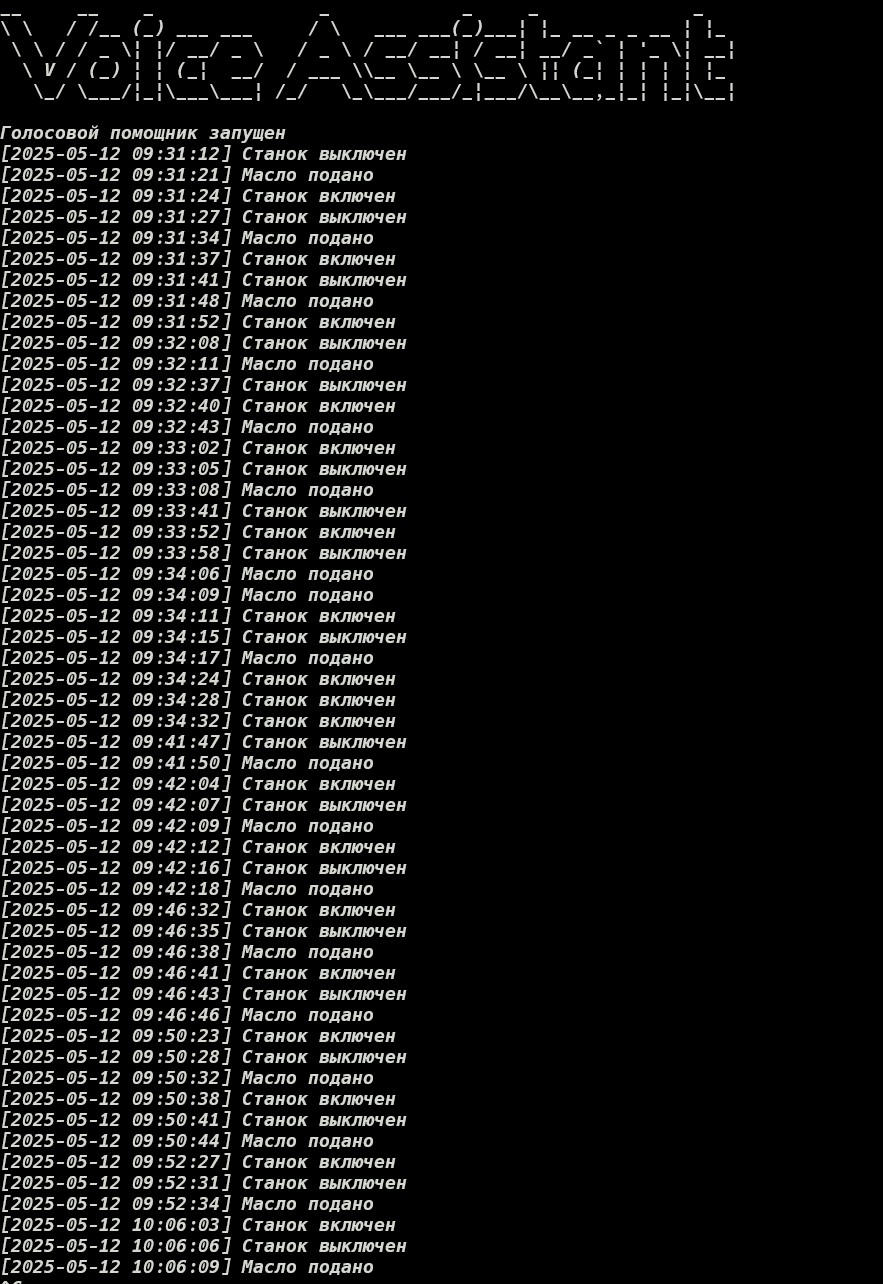
\includegraphics[scale=0.9]{test2_full.jpg}
	\caption{Название }
	\label{fig:test2}
\end{figure}

\subsection{Оценка эффективности}

Для объективного анализа нагрузки голосового помошника на одноплатный компьютер был проведён эксперимент с использованием двух поколений аппаратных платформ:
\begin{itemize}
	\item Raspberry Pi 2 Model B Rev 1.1;
	\item Raspberry Pi 4 Model B Rev 1.5.
\end{itemize}

\begin{figure}[H]
	\centering
	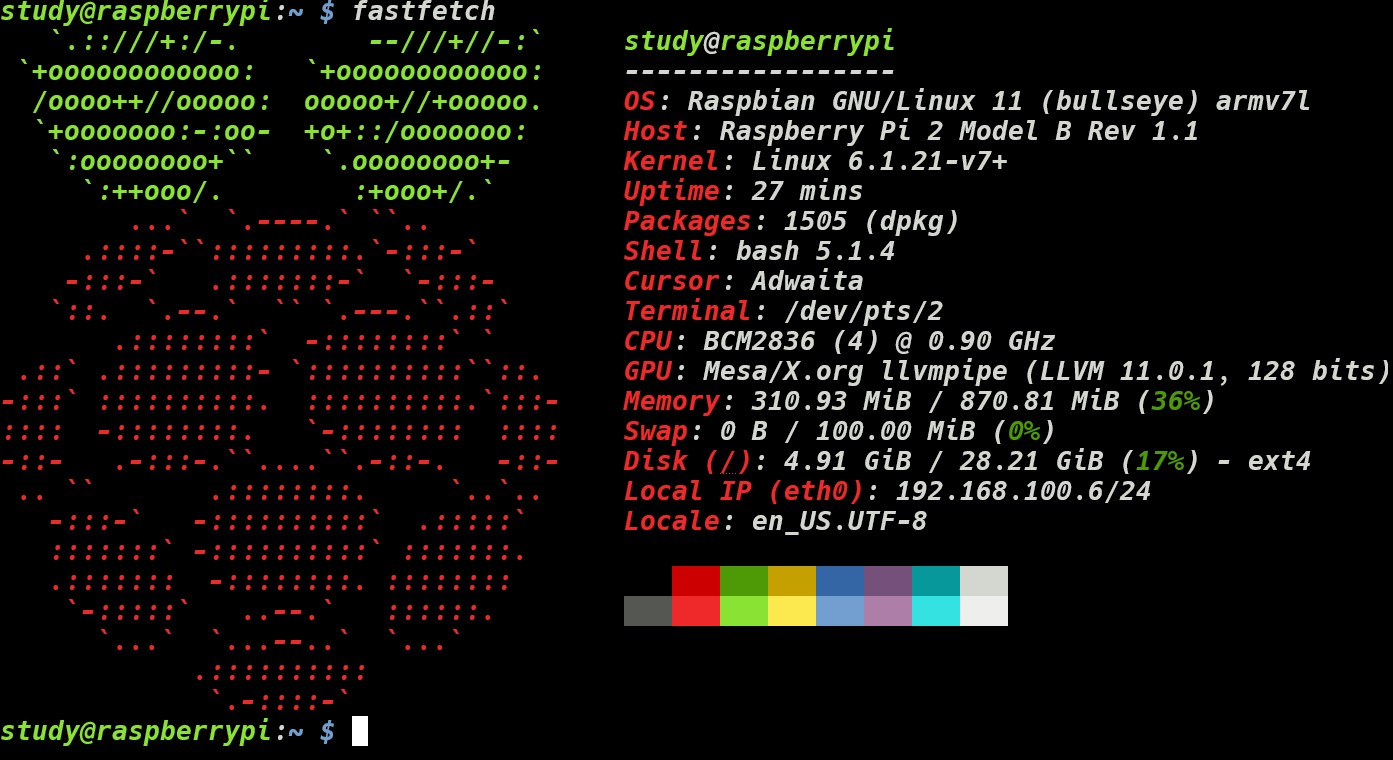
\includegraphics[scale=0.6]{fastfetch_RaspberryPi2.jpg}
	\caption{вывод программы fastfetch}
	\label{fig:fastfetch_RaspberryPi2}
\end{figure}


\begin{figure}[H]
	\centering
	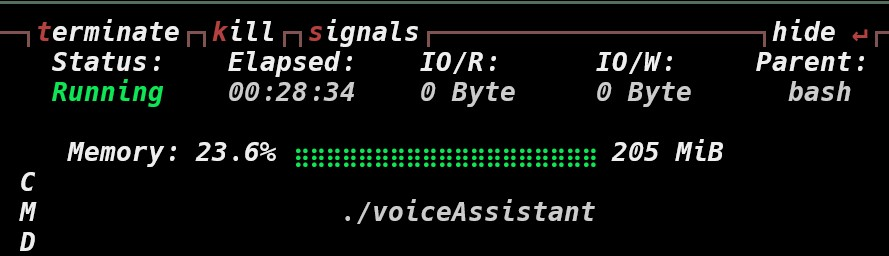
\includegraphics[scale=0.9]{useMemoryRaspberryPi2.jpg}
	\caption{вывод программы btop о используемой памяти голосовыйм помошником}
	\label{fig:useMemoryRaspberryPi2}
\end{figure}

\begin{table}[H]
	\caption{Используемые ресурсы при работе голосового помощника}
	\centering 
	\begin{tblr}{
			width=\textwidth,
			colspec={X[4,l]|X[1.5,c,m]|X[1.5,c,m]},
			cell{3-11}{1} = {l},  % Объединенные ячейки (строки 3-11, столбец 1) - по левому краю
			vlines,
		}
		\hline 
		\SetCell[r=2]{c} Модель одноплатного компьютера & \SetCell[c=2]{c} Используемые ресурсы
		&   \\ 
		\hline  
		& CPU & RAM \\
		\hline  
		1 Raspberry Pi 2 Model B Rev 1.1  & 10-20\%  & 205Mb  \\ 
		\hline  
		2 Raspberry Pi 4 Model B Rev 1.5 & 2-5\% & 205Mb \\ 
		\hline  
	\end{tblr}
\end{table}

\newpage
